\documentclass[aspectratio=169,11pt]{beamer}
\usepackage{beamerucad}
\usepackage{listings}
\definecolor{ckw}{HTML}{2563AB}\definecolor{cst}{HTML}{2E8B57}\definecolor{ccm}{HTML}{8A8F98}
\definecolor{outbg}{HTML}{F4F5F7}\definecolor{outrule}{HTML}{2E8B57}
\lstdefinestyle{py}{language=Python,basicstyle=\ttfamily\scriptsize,
 keywordstyle=\color{ckw}\bfseries,stringstyle=\color{cst},commentstyle=\color{ccm}\itshape,
 showstringspaces=false,columns=fullflexible,keepspaces=true,
 backgroundcolor=\color{ucadband!8},frame=leftline,framerule=2.5pt,rulecolor=\color{ucadband},
 xleftmargin=8pt,aboveskip=3pt,belowskip=1pt,basewidth=0.5em}
\lstdefinestyle{out}{basicstyle=\ttfamily\scriptsize\color{black!82},
 backgroundcolor=\color{outbg},frame=leftline,framerule=2.5pt,rulecolor=\color{outrule},
 xleftmargin=8pt,aboveskip=2pt,belowskip=1pt,columns=fullflexible,keepspaces=true}
\lstset{style=py}
\newcommand{\resultat}{{\scriptsize\textbf{R\'esultat}~$\rightarrow$}\par\vspace{1pt}}

\title{Programmation Python — Séance 8}
\subtitle{Visualiser et faire le pont}
\author{Dr. El Hadji Bassirou TOURÉ}
\institute{Département de Mathématiques et Informatique\\ Faculté des Sciences et Techniques\\ Université Cheikh Anta Diop de Dakar}
\date{}
\setucadfoot{Programmation Python — Séance 8}
\begin{document}

\begin{frame}[plain,noframenumbering]\titlepage\end{frame}

% =====================================================================
\begin{frame}{Objectifs de la séance}
\begin{ucaddef}[De quoi parle cette séance]
{\small Jusqu'ici, on a appris à \textbf{calculer} sur des données. Aujourd'hui, on apprend à les \textbf{regarder} — et à comprendre ce qu'un graphique dit, ou ne dit pas. C'est la dernière étape avant le Machine Learning.}
\end{ucaddef}
\begin{itemize}\small
  \item \textbf{Pourquoi} visualiser : ce qu'une moyenne ne montre pas.
  \item \textbf{Comment lire} un graphique : ses éléments, ce qu'on y cherche.
  \item \textbf{Lequel choisir} : histogramme, barres ou nuage de points.
  \item \textbf{Le pont vers le ML} : reconnaître un fruit à partir de ses mesures.
\end{itemize}
\end{frame}

\begin{frame}[fragile]{Le jeu de données : 30 fruits du marché}
\begin{ucaddef}[Trois fruits, trois mesures]
{\small On a pesé et mesuré 10 \textbf{mangues}, 10 \textbf{bananes} et 10 \textbf{oranges}. Pour chaque fruit : sa \textbf{masse} (g), sa \textbf{longueur} (cm) et son \textbf{taux de sucre} (\%).}
\end{ucaddef}
\begin{lstlisting}[style=out]
    fruit  masse  longueur  sucre
0  mangue    301      10.3   14.7
1  banane    137      18.4   11.1
2  orange    201       8.1    9.2
\end{lstlisting}
{\small \textbf{Une ligne = un fruit. Une colonne = une mesure.} C'est la forme de toute table de données, et celle que le Machine Learning attend.}
\end{frame}

% #####################################################################
\section{Pourquoi visualiser}

\begin{frame}{Le problème : une moyenne ne dit pas tout}
\begin{ucadfront}[Une question simple]
{\small Deux paniers de fruits ont \textbf{exactement la même masse moyenne} : 200 g. Contiennent-ils la même chose ?}
\end{ucadfront}
{\small Avec les seuls chiffres, impossible de répondre : la moyenne est identique. Il faut \textbf{regarder la répartition} — c'est-à-dire compter combien de fruits se trouvent dans chaque tranche de masse.}
\end{frame}

\begin{frame}{La réponse, en un coup d'œil}
\figslide{0.86}{figs/f8_meme_moyenne}{Deux paniers de masse moyenne identique (200 g), mais de composition totalement différente.}
\end{frame}

\begin{frame}{Ce que cette figure nous apprend}
\begin{itemize}\small
  \item \textbf{Panier A} : tous les fruits pèsent autour de 200 g. La moyenne \textbf{représente bien} le panier — ce sont sans doute dix oranges.
  \item \textbf{Panier B} : aucun fruit ne pèse 200 g ! Il y a des fruits légers ($\approx$ 120 g) et des fruits lourds ($\approx$ 280 g). La moyenne ne correspond à \textbf{aucun} fruit réel.
\end{itemize}
\begin{ucadret}[À retenir]
{\small Une moyenne résume, mais elle \textbf{cache la forme} des données. Deux jeux très différents peuvent avoir la même moyenne : \textbf{il faut regarder avant de conclure}.}
\end{ucadret}
\end{frame}

\begin{frame}{Ce qu'un graphique permet de voir}
\begin{itemize}\small
  \item \textbf{La répartition} : les valeurs sont-elles groupées, étalées, ou séparées en plusieurs paquets ?
  \item \textbf{Les groupes} : y a-t-il des familles distinctes dans les données ?
  \item \textbf{Les liens} : quand une mesure augmente, qu'arrive-t-il à une autre ?
  \item \textbf{Les anomalies} : une valeur aberrante saute aux yeux sur un graphique, jamais dans un tableau.
\end{itemize}
{\small C'est pourquoi visualiser est le \textbf{premier réflexe} de tout travail sur des données — avant le moindre calcul savant.}
\end{frame}

% #####################################################################
\section{Lire un graphique}

\begin{frame}{Les éléments d'un graphique}
\figslide{0.66}{figs/f8_anatomie}{Tout graphique se lit de la même façon : un titre, deux axes légendés, et des formes qui portent l'information.}
\end{frame}

\begin{frame}{Un graphique sans légende ne veut rien dire}
\begin{ucadpiege}[L'erreur la plus fréquente]
{\small Un graphique sans titre ni unités est \textbf{illisible} : « 300 » de quoi ? des grammes, des francs, des fruits ?}
\end{ucadpiege}
\begin{itemize}\small
  \item \texttt{title} : ce que l'on regarde.
  \item \texttt{xlabel} et \texttt{ylabel} : ce que représente chaque axe, \textbf{avec l'unité}.
  \item \texttt{legend} : à quoi correspond chaque couleur, dès qu'il y a des groupes.
\end{itemize}
{\small Trois lignes de code, mais elles font la différence entre une image et une \textbf{information}.}
\end{frame}

% #####################################################################
\section{Choisir le bon graphique}

\begin{frame}{Le graphique dépend de la question posée}
\figslide{0.9}{figs/f8_choisir}{On ne choisit pas un graphique parce qu'il est joli, mais parce qu'il répond à la question que l'on se pose.}
\end{frame}

\begin{frame}{Trois questions, trois graphiques}
\begin{itemize}\small
  \item « \textbf{Comment se répartissent les masses ?} » — une seule mesure, on veut sa forme : \textbf{histogramme}.
  \item « \textbf{Quel fruit est le plus lourd en moyenne ?} » — une mesure comparée entre groupes : \textbf{diagramme en barres}.
  \item « \textbf{Les fruits longs sont-ils les plus lourds ?} » — deux mesures ensemble : \textbf{nuage de points}.
\end{itemize}
\begin{ucadret}[La bonne habitude]
{\small Formuler la question \textbf{en français d'abord}. Le choix du graphique en découle, et le code n'est plus qu'une formalité.}
\end{ucadret}
\end{frame}

% #####################################################################
\section{L'histogramme}

\begin{frame}{Comprendre l'histogramme}
\begin{ucaddef}[L'idée en une phrase]
{\small L'histogramme découpe l'axe d'une mesure en \textbf{tranches} de même largeur, puis compte combien d'individus tombent dans chaque tranche. La hauteur d'une barre est donc un \textbf{effectif}.}
\end{ucaddef}
\begin{ucadfront}[Une image]
{\small Comme si l'on rangeait les fruits dans des casiers étiquetés « 100--120 g », « 120--140 g »... puis qu'on comptait les fruits de chaque casier.}
\end{ucadfront}
{\small Attention : les barres se touchent, car la mesure est \textbf{continue} — c'est ce qui le distingue du diagramme en barres.}
\end{frame}

\begin{frame}[fragile]{L'histogramme en pratique}
\begin{lstlisting}
plt.hist(df["masse"], bins=range(100, 360, 20))
plt.xlabel("masse (g)")
plt.ylabel("nombre de fruits")
plt.title("Distribution des masses")
\end{lstlisting}
\begin{center}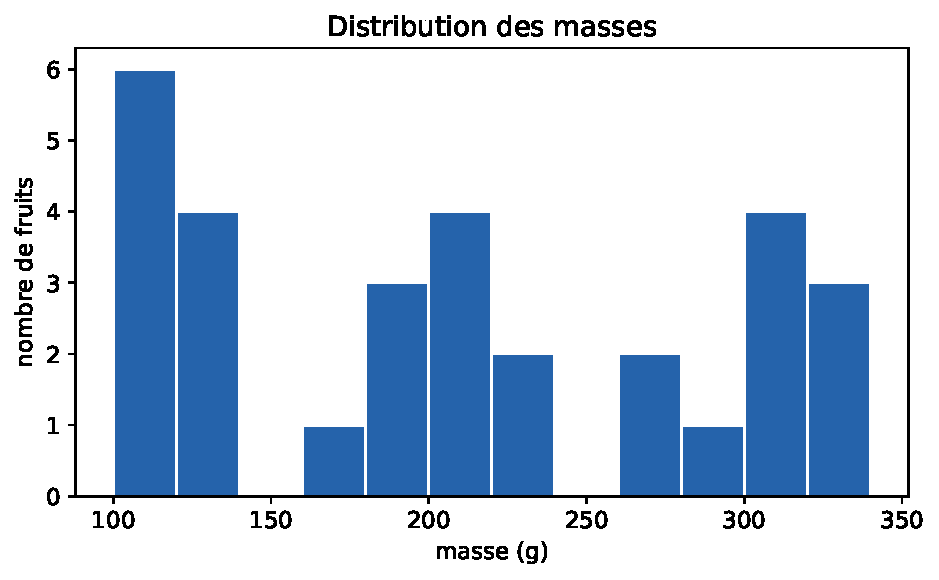
\includegraphics[height=0.40\textheight]{figs/f8_hist.pdf}\end{center}
\end{frame}

\begin{frame}{Lire cet histogramme}
\begin{itemize}\small
  \item L'axe des x porte la \textbf{masse} ; l'axe des y, le \textbf{nombre de fruits}.
  \item On distingue \textbf{trois amas} : vers 120 g, vers 200 g et vers 300 g.
  \item Entre ces amas, presque \textbf{aucun fruit} : les groupes sont bien séparés.
\end{itemize}
\begin{ucadret}[L'interprétation]
{\small Trois amas $=$ trois familles de fruits. Ce sont les \textbf{bananes}, les \textbf{oranges} et les \textbf{mangues} — alors que la colonne \texttt{fruit} n'a jamais été utilisée pour tracer ce graphique.}
\end{ucadret}
\end{frame}

\begin{frame}{Le rôle des tranches (\texttt{bins})}
\begin{itemize}\small
  \item Des tranches \textbf{trop larges} lissent tout : les trois amas disparaissent en une seule barre.
  \item Des tranches \textbf{trop fines} font apparaître du bruit : chaque fruit devient sa propre barre.
  \item On ajuste jusqu'à voir la \textbf{structure} sans le bruit — ici, des tranches de 20 g.
\end{itemize}
{\small C'est un \textbf{réglage}, pas une vérité : changer les tranches change ce que l'on voit. Raison de plus pour toujours indiquer ses choix.}
\end{frame}

% #####################################################################
\section{Le diagramme en barres}

\begin{frame}{Comprendre le diagramme en barres}
\begin{ucaddef}[L'idée en une phrase]
{\small Le diagramme en barres compare \textbf{une valeur entre des groupes} : une barre par groupe, dont la hauteur est la valeur. Il part toujours d'une \textbf{agrégation} — une moyenne, une somme, un comptage.}
\end{ucaddef}
{\small La démarche est en deux temps, déjà vus en Séance 7 :}
\begin{enumerate}\small
  \item \textbf{Regrouper puis résumer} : \texttt{groupby("fruit")["masse"].mean()}.
  \item \textbf{Tracer} le résultat : une barre par fruit.
\end{enumerate}
\end{frame}

\begin{frame}[fragile]{Le diagramme en barres en pratique}
\begin{lstlisting}
masse_moy = df.groupby("fruit")["masse"].mean()
plt.bar(masse_moy.index, masse_moy.values)
plt.ylabel("masse moyenne (g)")
plt.title("Masse moyenne par fruit")
\end{lstlisting}
\begin{center}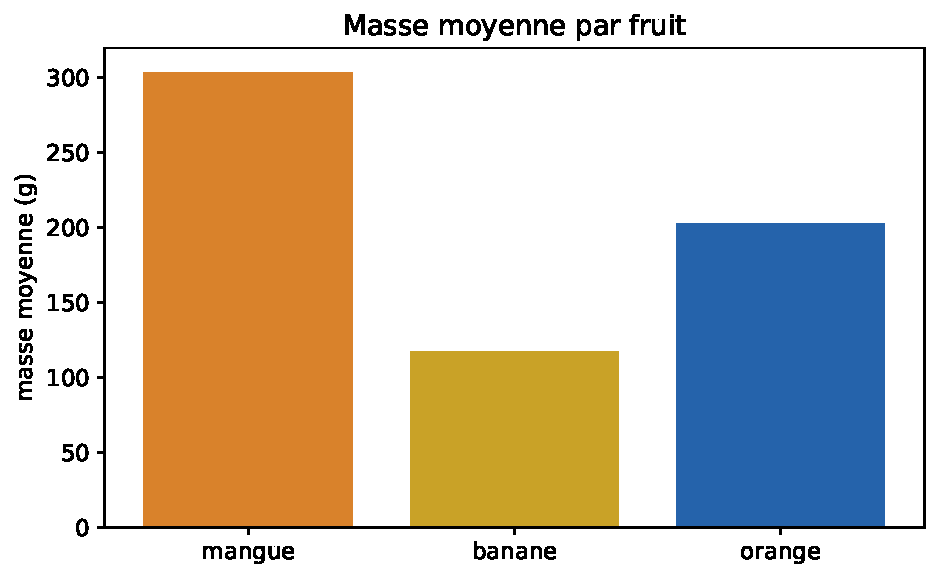
\includegraphics[height=0.38\textheight]{figs/f8_bar.pdf}\end{center}
\end{frame}

\begin{frame}{Lire ce diagramme}
\begin{ucadret}[Les chiffres]
{\small Mangue : \textbf{304 g} en moyenne. Orange : \textbf{204 g}. Banane : \textbf{119 g}.}
\end{ucadret}
\begin{itemize}\small
  \item La comparaison est \textbf{immédiate} : une mangue pèse environ deux fois et demie une banane.
  \item Mais attention : ce graphique montre des \textbf{moyennes}. Il ne dit rien de la dispersion à l'intérieur de chaque groupe.
\end{itemize}
{\small C'est le complément de l'histogramme, pas son remplaçant : l'un montre la \textbf{forme}, l'autre compare des \textbf{résumés}.}
\end{frame}

% #####################################################################
\section{Le nuage de points}

\begin{frame}{Comprendre le nuage de points}
\begin{ucaddef}[L'idée en une phrase]
{\small Le nuage de points place chaque individu selon \textbf{deux} mesures : une en abscisse, une en ordonnée. Chaque point est un fruit ; sa position résume ses deux mesures.}
\end{ucaddef}
{\small On y cherche deux choses :}
\begin{itemize}\small
  \item un \textbf{lien} : quand la longueur augmente, la masse augmente-t-elle aussi ?
  \item des \textbf{groupes} : les points forment-ils des paquets séparés ?
\end{itemize}
{\small En \textbf{colorant par catégorie}, on répond aux deux questions d'un seul regard.}
\end{frame}

\begin{frame}{Le nuage révèle les fruits}
\figslide{0.55}{figs/f8_scatter}{Chaque point est un fruit, placé selon sa longueur et sa masse, coloré selon son type.}
\vspace{-3pt}
{\small Trois \textbf{amas nettement séparés}, sans le moindre chevauchement.}
\end{frame}

\begin{frame}{Lire ce nuage, groupe par groupe}
\begin{itemize}\small
  \item La \textbf{banane} : longue (17--20 cm) mais légère ($\approx$ 120 g) — en bas à droite.
  \item La \textbf{mangue} : courte (10--12 cm) et lourde ($\approx$ 300 g) — en haut au milieu.
  \item L'\textbf{orange} : la plus courte (7--9 cm), de masse moyenne ($\approx$ 200 g) — à gauche.
\end{itemize}
\begin{ucadret}[Le point décisif]
{\small Les trois groupes ne se touchent pas. Autrement dit : \textbf{connaître la longueur et la masse suffit à identifier le fruit} — sans le voir. C'est exactement ce que le Machine Learning va automatiser.}
\end{ucadret}
\end{frame}

% #####################################################################
\section{Une mini-EDA}

\begin{frame}{La démarche d'analyse exploratoire}
\begin{ucaddef}[Quatre gestes, toujours les mêmes]
{\small L'\textbf{analyse exploratoire} (EDA) n'est pas une technique, c'est une \textbf{méthode} : comprendre les données avant de modéliser.}
\end{ucaddef}
\begin{enumerate}\small
  \item \textbf{Charger} : lire le fichier, vérifier \texttt{shape} — combien de lignes, de colonnes ?
  \item \textbf{Décrire} : \texttt{describe}, \texttt{value\_counts} — quelles valeurs, quels effectifs, des manques ?
  \item \textbf{Tracer} : histogramme, barres, nuage — quelle forme, quels groupes ?
  \item \textbf{Observer} : formuler en français ce que l'on a compris.
\end{enumerate}
\end{frame}

\begin{frame}[fragile]{Le profil de chaque fruit}
\begin{lstlisting}
print(df.groupby("fruit")[["masse", "longueur", "sucre"]].mean().round(1))
\end{lstlisting}
\resultat
\begin{lstlisting}[style=out]
        masse  longueur  sucre
fruit
banane  119.0      19.0   11.8
mangue  304.4      10.9   14.0
orange  204.3       8.2    9.0
\end{lstlisting}
{\small Trois lignes, trois colonnes : le \textbf{portrait chiffré} de chaque fruit.}
\end{frame}

\begin{frame}{L'étape « observer » : que dit ce tableau ?}
\begin{itemize}\small
  \item La \textbf{mangue} est la plus lourde (304 g) et la plus sucrée (14 \%).
  \item La \textbf{banane} est de loin la plus longue (19 cm) et la plus légère.
  \item L'\textbf{orange} est la moins sucrée (9 \%) et la plus courte.
\end{itemize}
\begin{ucadret}[Le point clé]
{\small \textbf{Chaque mesure sépare les fruits, à sa manière.} La masse distingue bien la mangue ; la longueur, la banane ; le sucre, l'orange. Un modèle exploitera les trois \textbf{ensemble}.}
\end{ucadret}
\end{frame}

% #####################################################################
\section{Le pont vers le ML}

\begin{frame}{L'idée du Machine Learning, en une image}
\begin{ucadfront}[Ce que l'on vient de faire à la main]
{\small En regardant le nuage de points, \textbf{vous} avez appris à reconnaître un fruit : « long et léger $\rightarrow$ banane ». Le Machine Learning, c'est confier cet apprentissage à un programme.}
\end{ucadfront}
{\small Pour cela, on lui donne les données sous une forme précise :}
\begin{itemize}\small
  \item \textbf{\texttt{X}} — ce que l'on \textbf{observe} : les mesures (masse, longueur, sucre).
  \item \textbf{\texttt{y}} — ce que l'on veut \textbf{prédire} : le nom du fruit.
\end{itemize}
\end{frame}

\begin{frame}{De la table aux objets \texttt{X} et \texttt{y}}
\figslide{0.66}{figs/f8_xy}{Les colonnes de mesures forment \texttt{X} ; la colonne à prédire forme \texttt{y}.}
\vspace{-3pt}
{\small Une ligne de \texttt{X} et la valeur de \texttt{y} en face décrivent \textbf{le même fruit}.}
\end{frame}

\begin{frame}[fragile]{Construire \texttt{X} et \texttt{y}}
\begin{lstlisting}
X = df[["masse", "longueur", "sucre"]].values
y = df["fruit"].values
print("X shape :", X.shape)
print("y shape :", y.shape)
\end{lstlisting}
\resultat
\begin{lstlisting}[style=out]
X shape : (30, 3)
y shape : (30,)
\end{lstlisting}
{\small \texttt{X} est une \textbf{matrice} \texttt{(30, 3)} : 30 fruits en lignes, 3 mesures en colonnes. \texttt{y} est un \textbf{vecteur} \texttt{(30,)} : un nom par fruit. Les deux ont forcément \textbf{le même nombre de lignes}.}
\end{frame}

\begin{frame}[fragile]{La suite, dans le cours de Machine Learning}
{\small Sous cette forme, \texttt{X} et \texttt{y} sont exactement ce qu'attend scikit-learn. Ce code n'est pas exécuté ici — il montre où l'on va :}
\begin{lstlisting}
modele = DecisionTreeClassifier()
modele.fit(X, y)                   # il APPREND le lien X -> y
modele.predict([[300, 11, 14]])    # 300 g, 11 cm, 14 % : mangue ?
\end{lstlisting}
\begin{ucadret}[Deux mots pour finir]
{\small \texttt{fit} : le modèle \textbf{apprend} sur des fruits déjà étiquetés. \texttt{predict} : il \textbf{décide} pour un fruit nouveau. Tout le cours de Machine Learning consiste à comprendre ce qui se passe entre les deux.}
\end{ucadret}
\end{frame}

% #####################################################################
\section{Synthèse}

\begin{frame}{Pièges fréquents}
\begin{itemize}\small
  \item \textbf{Conclure sur une moyenne} sans avoir regardé la répartition (souvenez-vous des deux paniers).
  \item \textbf{Oublier les légendes} : un graphique sans titre ni unités n'informe personne.
  \item \textbf{Choisir le graphique avant la question} : c'est la question qui commande.
  \item \textbf{Confondre les rôles} : \texttt{X} contient ce que l'on mesure, \texttt{y} ce que l'on cherche à prédire.
\end{itemize}
\end{frame}

\begin{frame}{À retenir — Séance 8}
\begin{ucadret}[L'essentiel]
{\small
\textbf{Pourquoi} : une moyenne cache la forme des données ; un graphique la révèle.\\[3pt]
\textbf{Lequel} : une mesure $\rightarrow$ histogramme ; une mesure par groupe $\rightarrow$ barres ; deux mesures $\rightarrow$ nuage de points.\\[3pt]
\textbf{Comment lire} : titre, axes légendés avec unités, légende des couleurs ; puis chercher formes, groupes, liens.\\[3pt]
\textbf{Mini-EDA} : charger $\rightarrow$ décrire $\rightarrow$ tracer $\rightarrow$ observer.\\[3pt]
\textbf{Pont ML} : \texttt{X} (ce que l'on mesure) et \texttt{y} (ce que l'on prédit) ; \texttt{fit} pour apprendre, \texttt{predict} pour décider.}
\end{ucadret}
\end{frame}

\begin{frame}{Bilan du cours}
\begin{ucaddef}[Le chemin parcouru]
{\small Des valeurs et des types (S1) aux structures (S2), au contrôle du flux (S3), aux fonctions (S4), aux objets (S5) ; puis à \texttt{NumPy} (S6), \texttt{pandas} (S7) et à la visualisation (S8).}
\end{ucaddef}
{\small Vous savez désormais \textbf{charger, explorer, résumer et représenter} des données — et vous comprenez ce qu'un modèle attend. Le cours de \textbf{Machine Learning} peut commencer.}
\end{frame}

\begin{frame}{Références}
\begin{itemize}\small
  \item Hunter, J. D. — \emph{Matplotlib: A 2D Graphics Environment}, CiSE, 2007.
  \item VanderPlas, J. — \emph{Python Data Science Handbook}, 2e éd., O'Reilly, 2023.
  \item McKinney, W. — \emph{Python for Data Analysis}, 3e éd., O'Reilly, 2022.
  \item Tufte, E. — \emph{The Visual Display of Quantitative Information}, 2e éd., 2001.
\end{itemize}
\end{frame}

\end{document}
